\documentclass{scrreprt}

\usepackage[german]{babel}
\usepackage{fourier}
\usepackage[utf8]{inputenc}
\usepackage[T1]{fontenc}
\usepackage{amsfonts,amsthm, amsmath}
\usepackage{listings}
% The following is needed in order to make the code compatible
% with both latex/dvips and pdflatex.
\ifx\pdftexversion\undefined
\usepackage[dvips]{graphicx}
\else
\usepackage[pdftex]{graphicx}
\DeclareGraphicsRule{*}{mps}{*}{}
\fi

\setlength\parindent{0pt}
\lstset{language=Erlang}

\begin{document}

\textbf{Team:} Falco Winkler (FW), Daniel Schruhl (DS)\\
\\
\textbf{Aufgabenteilung:}\\

\textbf{Quellenangaben:}\\
\\
\textbf{Bearbeitungszeitraum:}
\begin{itemize}
	\item 26.03.2017 (FW,DS)
\end{itemize}

\textbf{Aktueller Stand:}\\

\textbf{Änderung des Entwurfs:}\\

\textbf{Entwurf:}\\
Sequenzdiagramm
\begin{figure}[!htb]
\centering
	\includegraphics[width=\textwidth]{sequence-diagram.png}
\caption[seq-dia]{Sequenzdiagramm bei fehlerfreiem Nachrichtenaustausch}
\label{fig:sequence-diagram}
\end{figure}

Komponentendiagramm
\begin{figure}[!htb]
\centering
	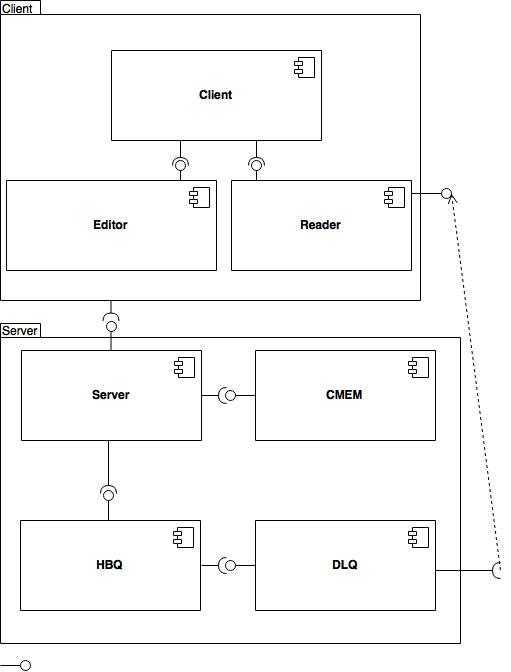
\includegraphics[width=\textwidth]{component-diagram.png}
\caption[seq-dia]{Komponentendiagramm der Message Of The Day App}
\label{fig:component-diagram}
\end{figure}

Das Softwareprodukt besteht aus mehreren Modulen und Paketen. Das Client-Paket und das Server-Paket.

Im Server Paket befinden sich das Server-Modul und alle vom Server-Modul verwendeten Datenstrukturen in Modulen.
Dazu gehören das HBQ-Modul, das DLQ-Modul und das CMEM-Modul.

Die Schnittstellen des DLQ-Moduls und CMEM-Moduls sind als RPC implementiert. Die Schnittstellen des HBQ-Moduls und des
Server-Moduls sind als entfernte ADT realisiert.

Die DLQ Schnittstelle wird nur von der HBQ konsumiert und die CMEM Schnittstelle wird nur vom Server konsumiert.
Die Schnittstelle der HBQ wird nur vom Server verwendet und die Schnittstelle vom Server ist nur an den Client angebunden.

Das Client-Paket beinhaltet die Client-Module. Diese sind zum einen der Lese Client (Reader-Modul) und der Redakteur
Client (Editor-Modul). Beide Clients sind als ein Prozess implementiert.

\end{document}